Dieses Szenario dient der Beobachtung der Flexibilität der Agenten. Außerdem soll der Unterschied zu einem zentralen Ansatz deutlich gemacht werden und die Skalierbarkeit des Ansatzes gezeigt werden.

\textbf{Aufbau des Experiments}
\begin{figure}[H]
    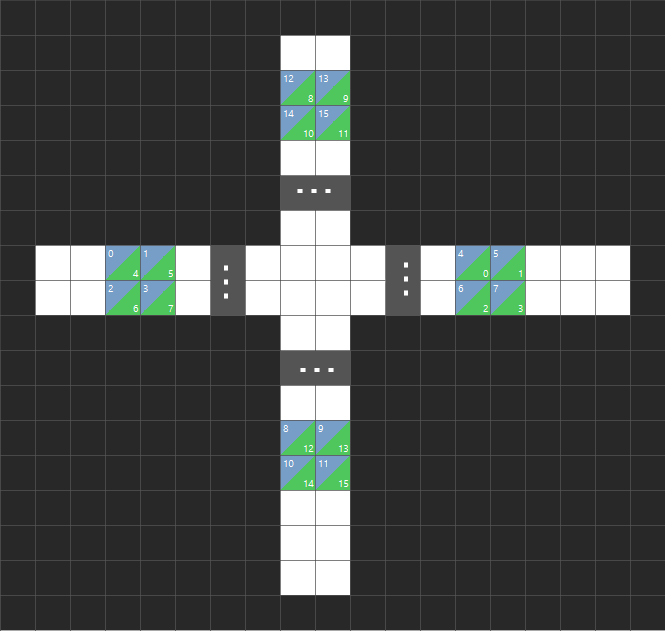
\includegraphics[width=\textwidth]{images/junction.png}
    \centering
    \caption{Aufbau für das Passieren einer Kreuzung von vier Gruppen, bestehend aus jeweils vier Agenten}
    \label{fig:kreuzung}
\end{figure}
In diesem Experiment versuchen vier Gruppen von jeweils vier Agenten eine Kreuzung zu durchqueren. Ziel jeder Gruppe ist es, die gegenüberliegende Seite in gleicher Formation zu erreichen. Der Kreuzungsbereich besteht aus acht freien Feldern, bietet also nicht genügend Platz für alle Agenten. Normale Verkehrsregeln, zum Beispiel das Rechtsfahrgebot, Vorfahrtsregeln oder das Bilden von Fahrspuren, sind keine Lösungen, die ein konfliktfreies aneinander Vorbeifahren der Agenten ermöglichen. Die vier Fahrbahnen der Kreuzung sind jeweils zwei Felder breit und 14 Felder lang.

\textbf{Erwartete Beobachtungen}\newline
Wegen der dynamischem Prioritäten ist eine Vielzahl an Lösungen zu beobachten. Der Berechnungsaufwand pro Agent steigt, trotz der gestiegenen Teilnehmerzahl, nicht.
Ein möglicher zentraler Ansatz würde vermutlich zwei Gruppen blockieren und die übrigen gegenüberliegenden Gruppen durch die Kreuzung passieren lassen, um erst danach den blockierten Gruppen die Durchfahrt zu gewähren. Dies ist vergleichbar mit einer Ampel an einer Kreuzung im Straßenverkehr.

